\subsection{Hardware}
The end system has two arrays, each with three microphones mounted on the vertices of a $20$ cm equilateral triangle. We used omni-directional foil electret condenser microphone due to its low cost and small size. The microphone has a frequency range of $100$ to $10K$ Hz, and a minimum SNR of 58dB\cite{sys:1}. We also used operational amplifer OPA344 from Texas Instrument to amplify the microphone output by a factor of 100, so the received signal can be easily picked up by the analog-to-digital converter (ADC) module installed on the micro-controller. The micro-controller board used in this project is \emph{teensy 3.1}, and it is attached to one of the vertices of the triangle. Fig~\ref{fig:setup_array} shows a picture of the array setup.  The micro-controller contains an onboard RAM of $64$k, and an ADC module capable of sampling at $500$kHz~\cite{tdoa:micloc, sys:teensy}. In this project, the micro-controller collects microphone data on all three channels for a duration $12$ milliseconds and then sends the recorded data to a computer through the USB port for localization. 

\begin{figure}[h!]
  \centering
  \begin{subfigure}[]{.48\textwidth}
    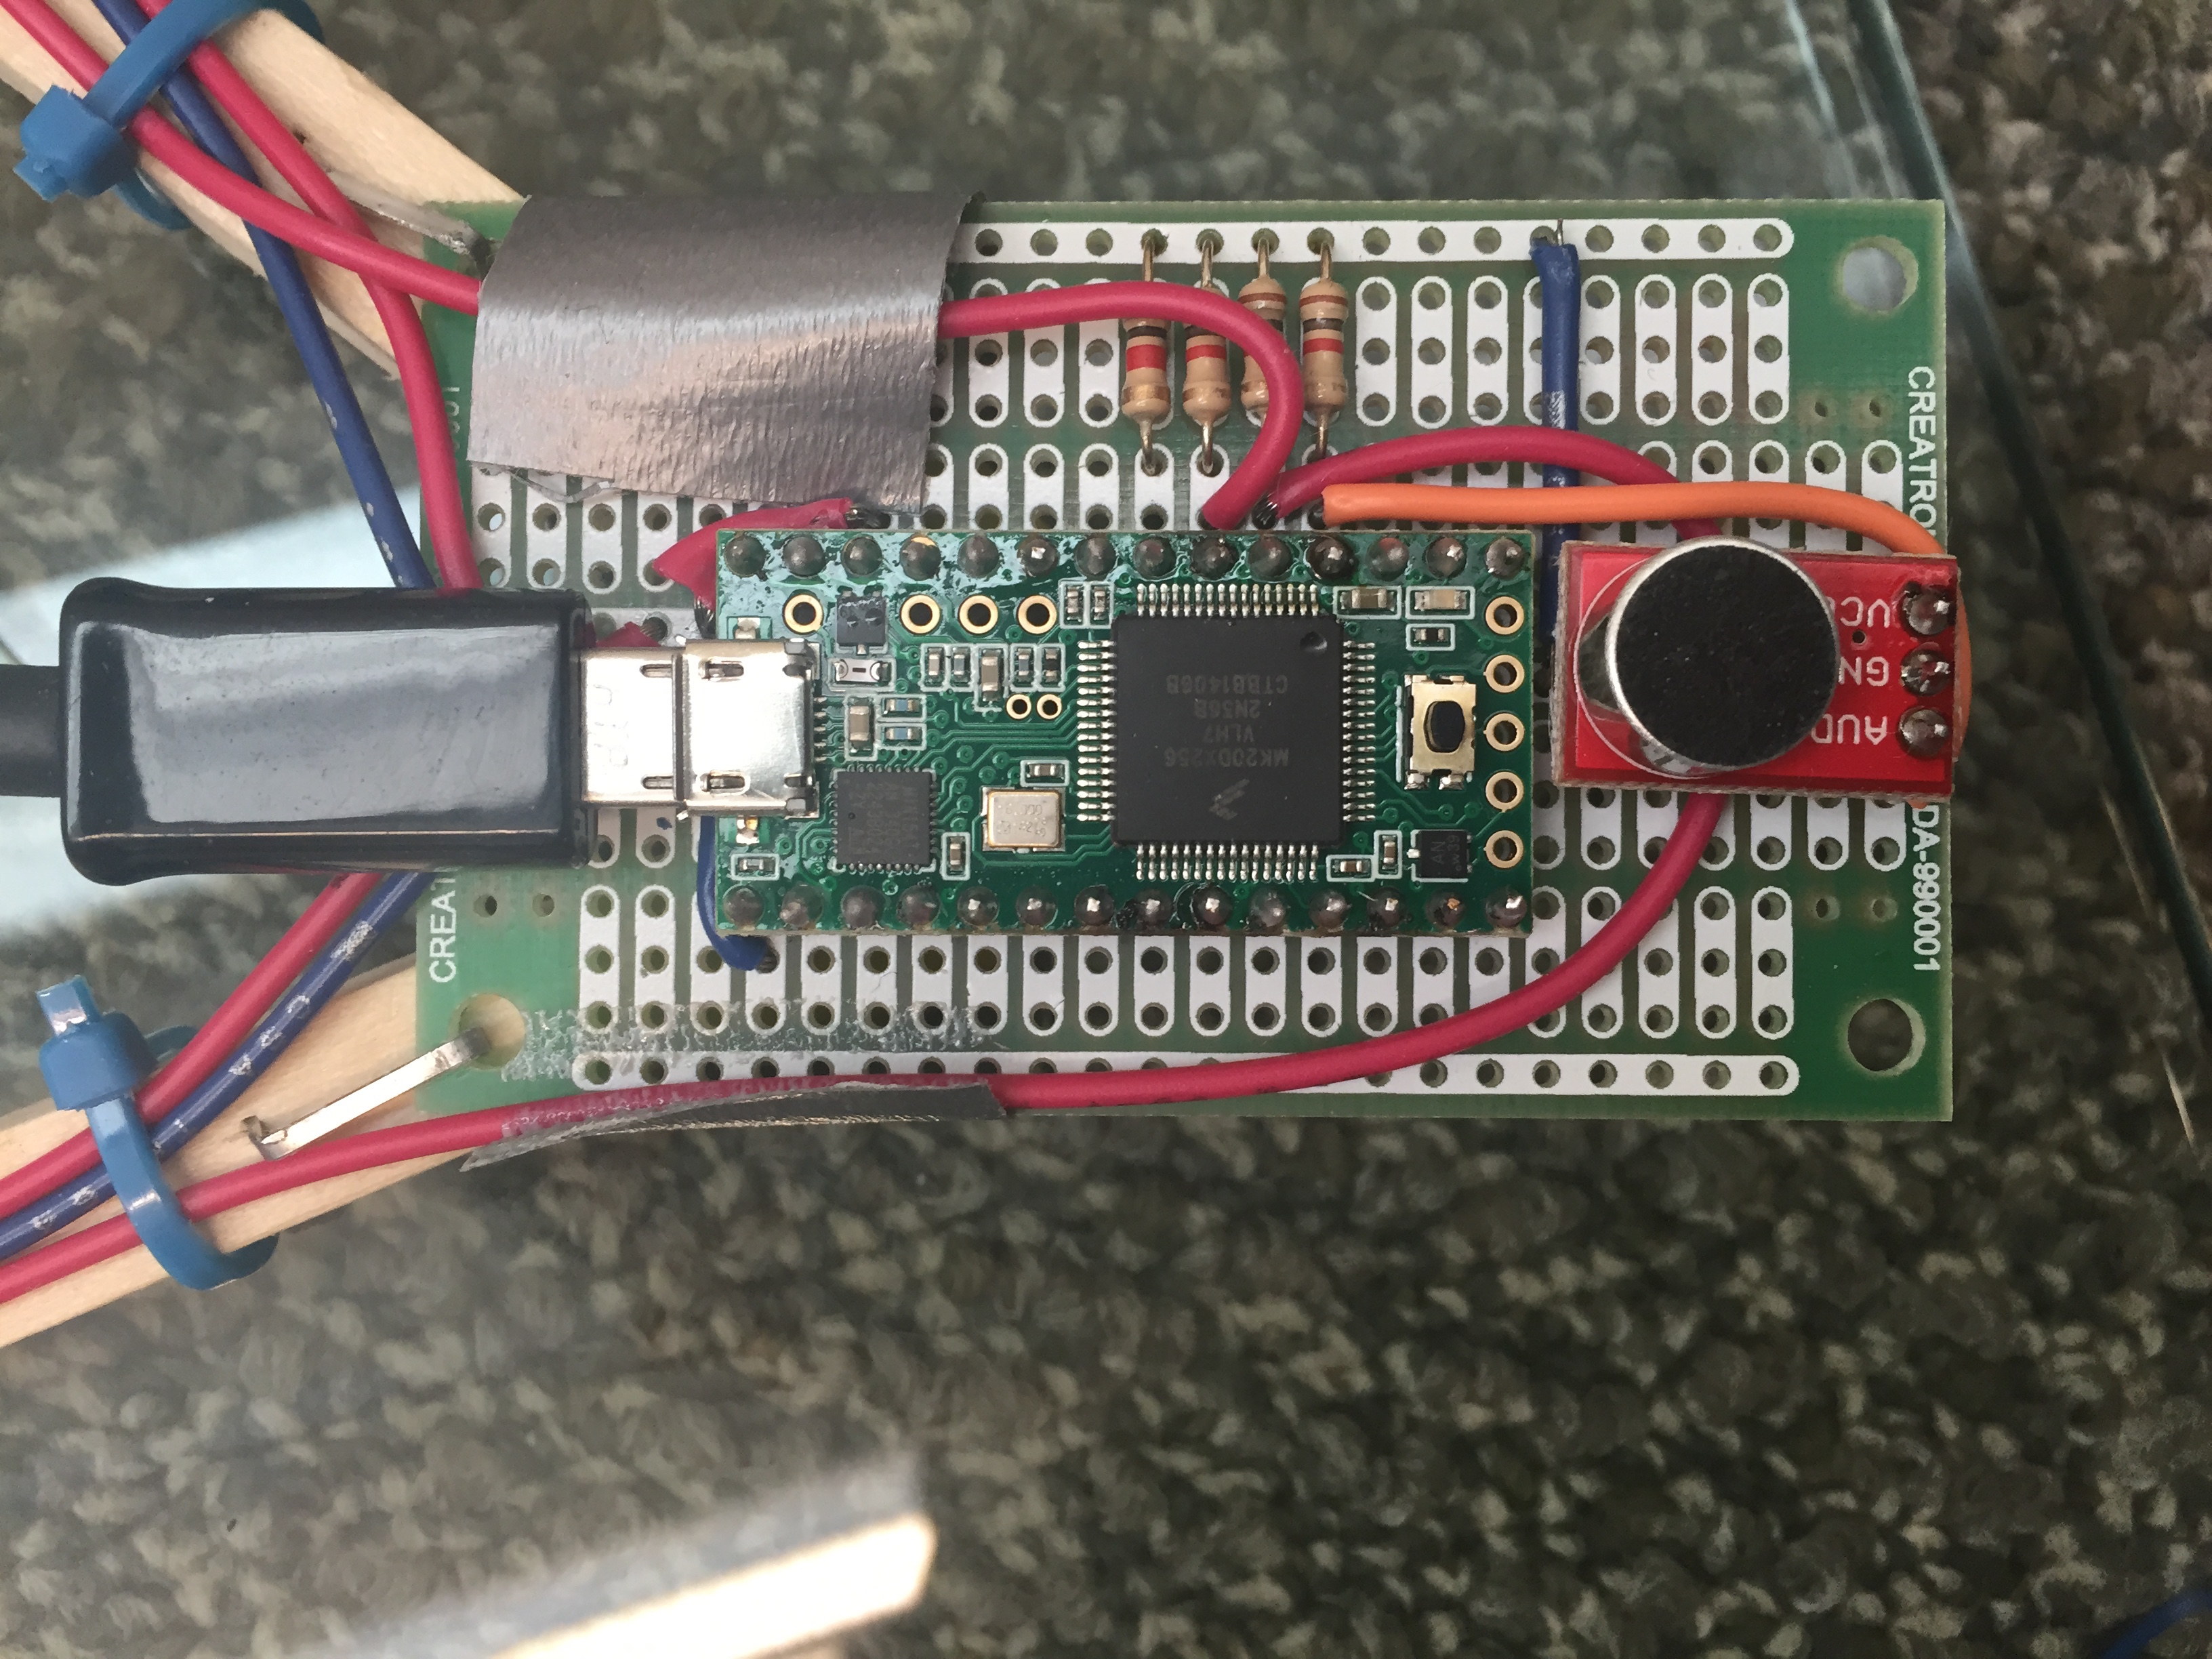
\includegraphics[width=\textwidth]{array_close.JPG}
    \caption{micro-controller}
  \end{subfigure}
  \begin{subfigure}[]{.48\textwidth}
    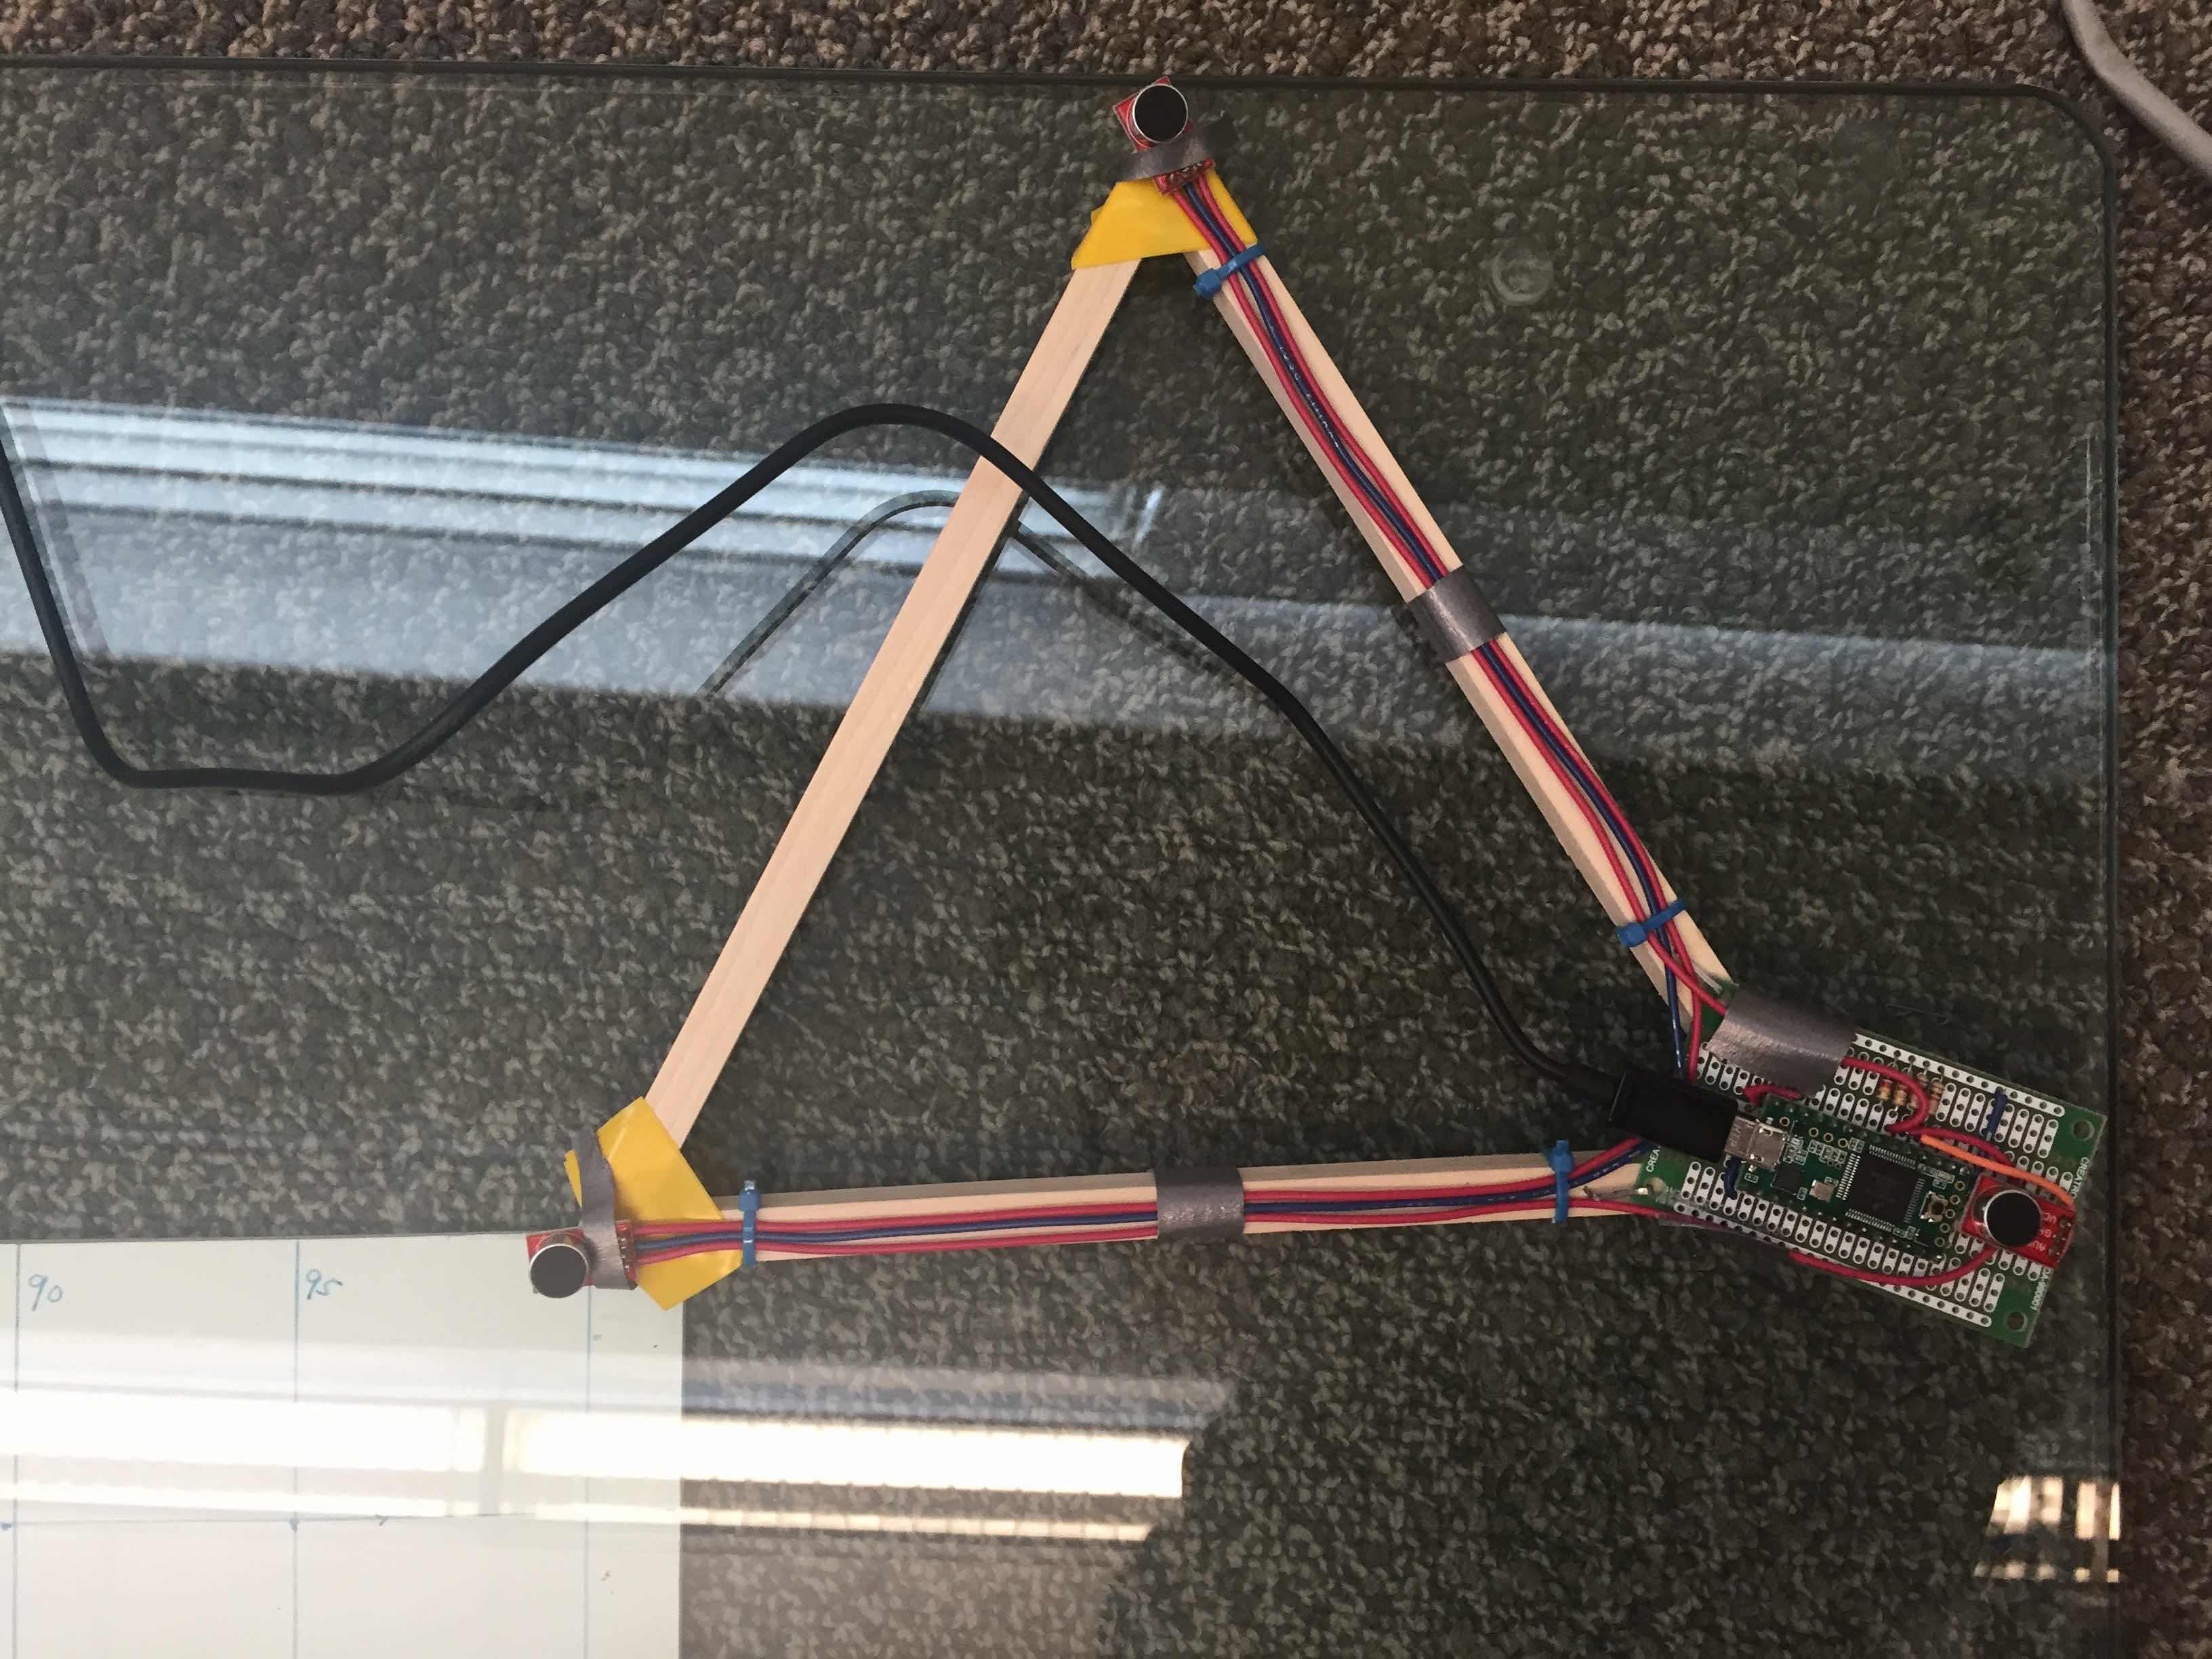
\includegraphics[width=\textwidth]{array.JPG}
    \caption{array}
  \end{subfigure}
  \begin{subfigure}[]{.48\textwidth}
    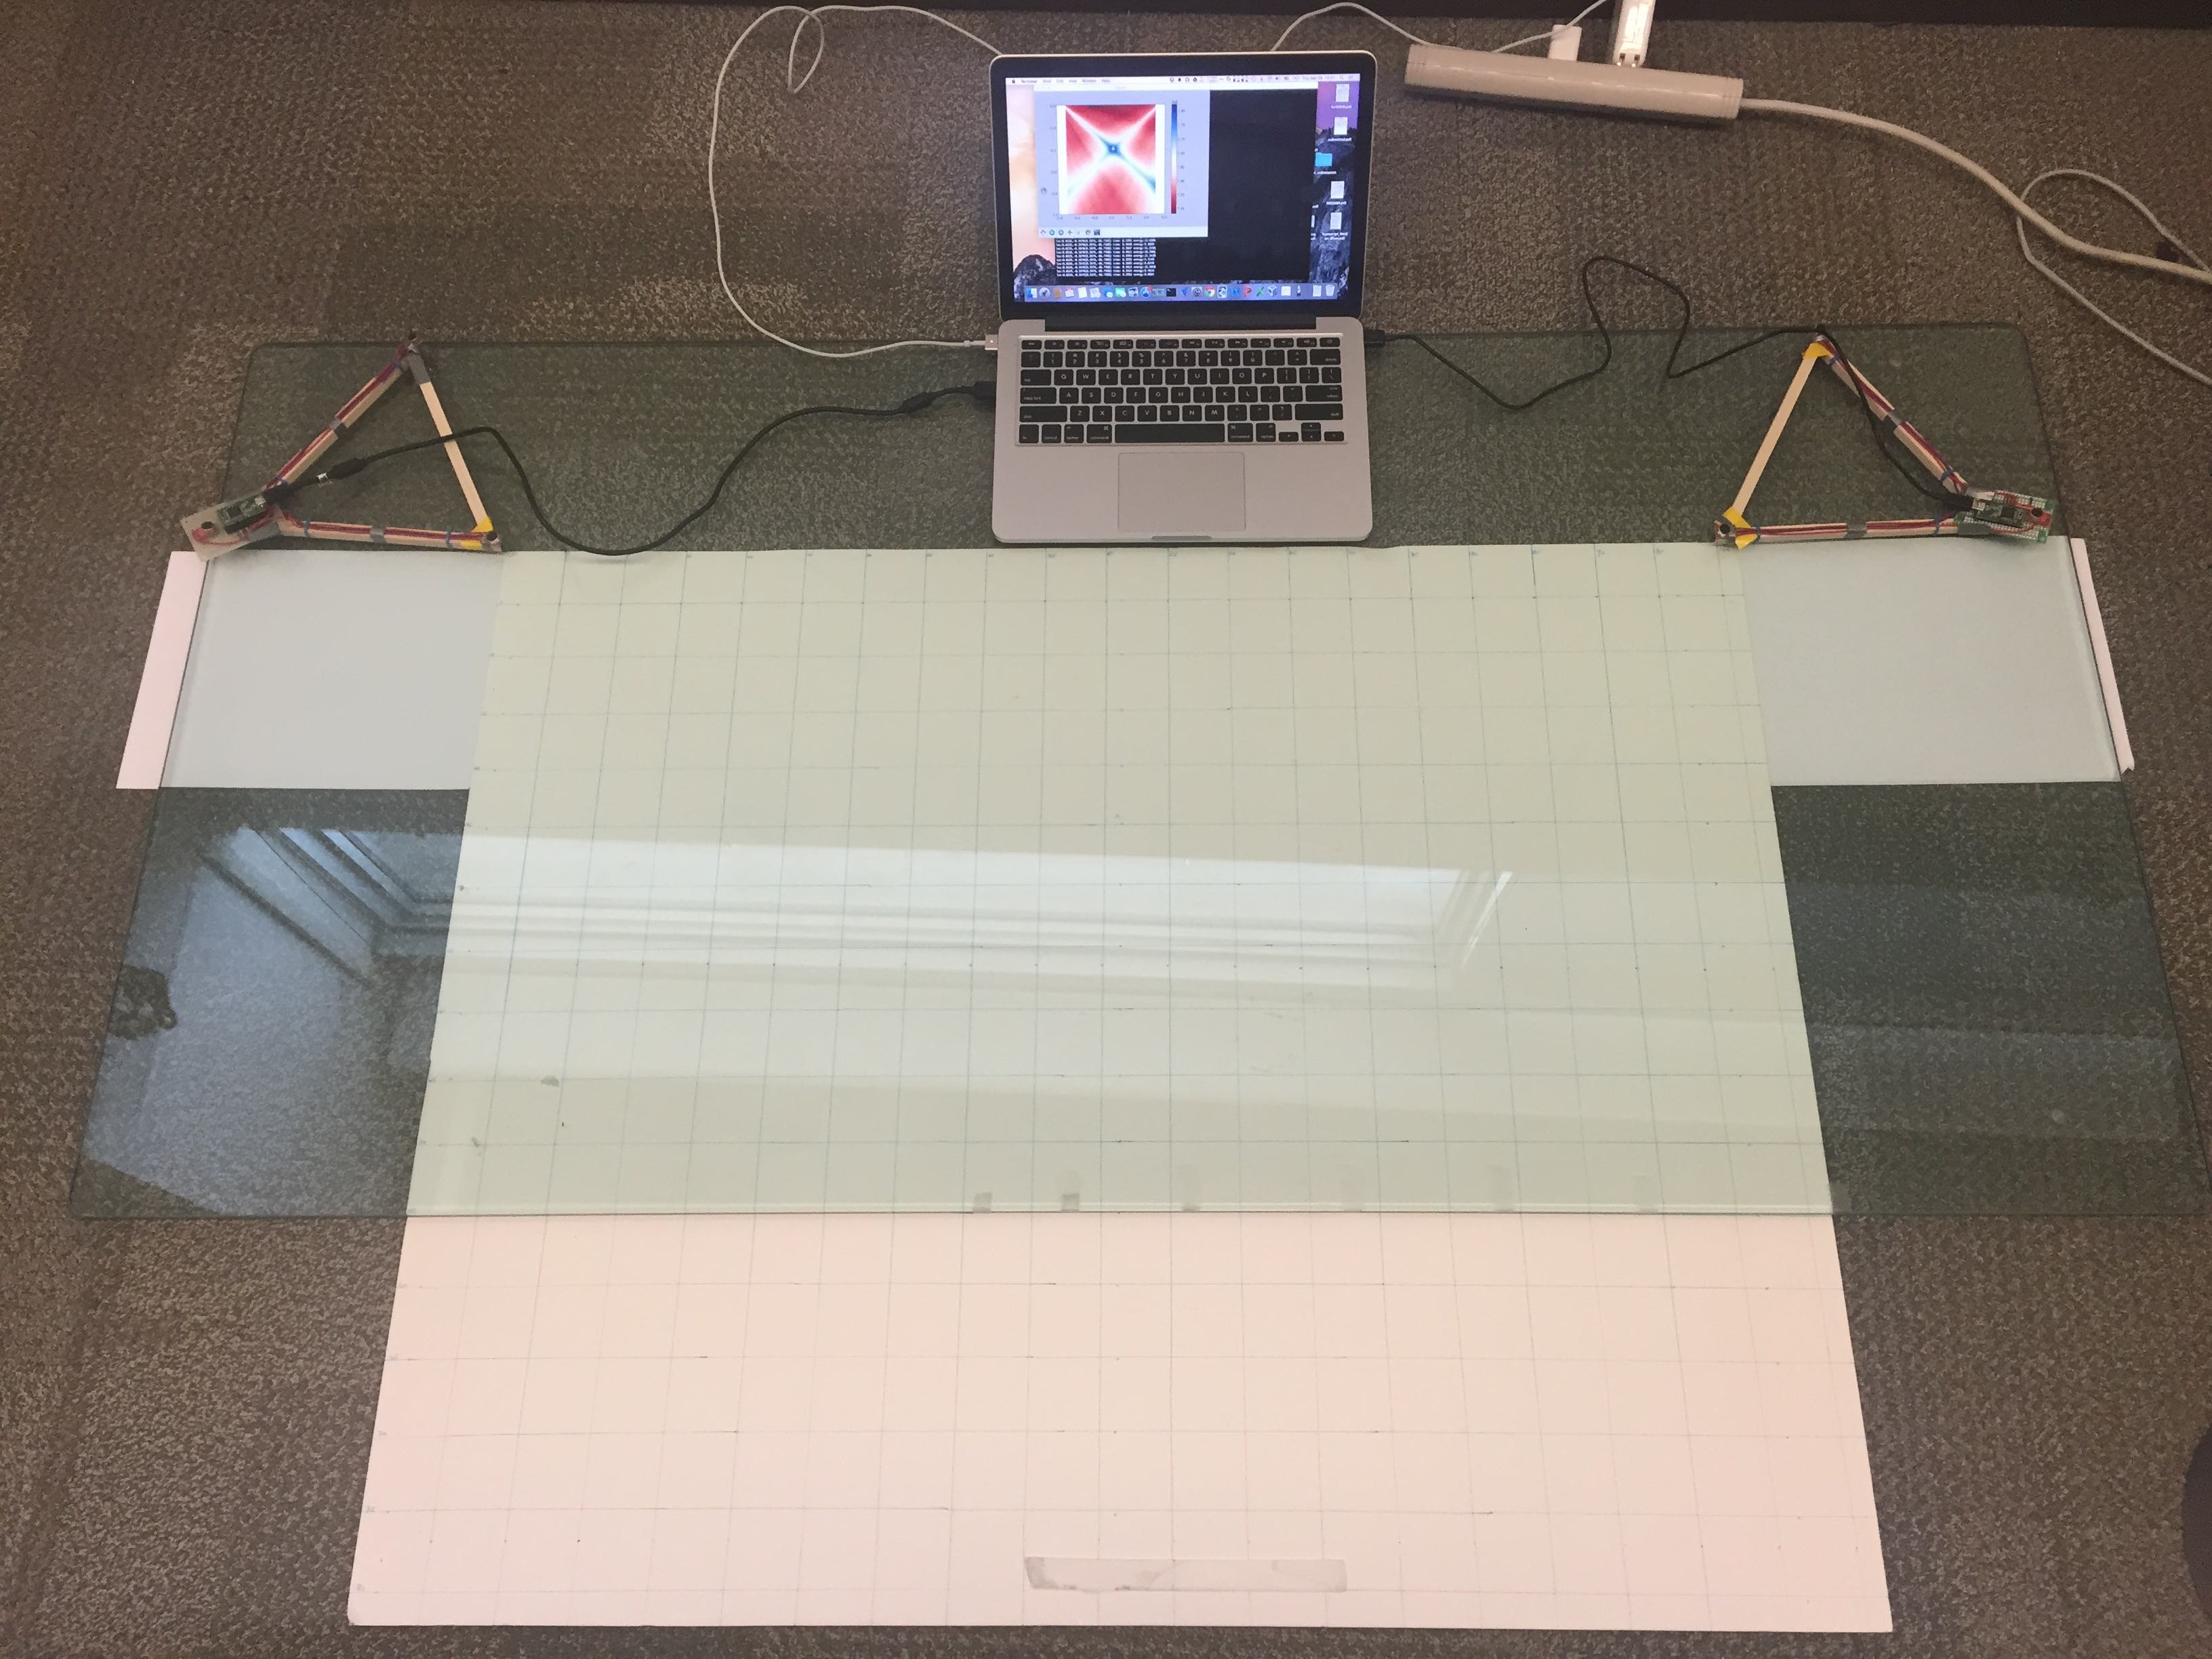
\includegraphics[width=\textwidth]{setup_2.JPG}
    \caption{two arrays}
  \end{subfigure}
  \caption{Localization system setup}
  \label{fig:setup_array}
\end{figure}

\subsection{Software}

On the software side, \emph{Python} is used as the main programming language since it has extensive libraries in both real time data handling and signal processing. \emph{ZeroMQ} is an inter process messaging queue that is used in our system to pass data across different modules. Our system is made up of two data acquisition modules (each is used to receive raw date from microphone array output) and one localization module (listens to both data acquisition modules and perform localization using the raw microphone data). Using ZeroMQ as connections to different modules adds flexibility to our system, as we can design applications such as the drawing application we have used in our system to interface only with the localization module and disregard how the microphone data is collected. Other localization applications can be easily integrated into our system by connecting them with the localization module. Furthermore, we have built a recording module that interfaces with the data acquisition modules for offline analysis and parameter tuning. 

To handle the uncertainty in TDOA estimation, instead of using point estimate that maximizes equation~\ref{eq:gcc}, we take the cross-correlation output(equation~\ref{eq:gcc2}) as a measure of the likelihood of different arrival time differences. Each index $i$ from the cross-correlation vector denotes the time delay across the two microphones receiving the acoustic signal, and the cross-correlation value $k$[i] at each index $i$ denotes the likelihood of the time delay being $i$. 

For each microphone array, we build a heatmap of likelihood for the region. The intensity at each point on the heatmap represents the likelihood of it being the source. To generate the likelihood heatmap for an microphone array, we apply the following algorithm. For each point ($x$,$y$) on the grid, the theoretical TDOA to each microphone pair can be precomputed using:
\[
 D_{m_1,m_2}(x,y) =  \frac{((x-x_1)^2 + (y-y_1)^2)^{0.5} - ((x-x_2)^2 + (y-y_2)^2)^{0.5}}{v}
\]
where ($x_1, y_1$) and ($x_2, y_2$) are the locations of the microphone pair and $v$ is the speed of sound. Then the heatmap can be generated by going through all the points on the grid and performing a lookup using equation~\ref{eq:gcc2}. With three microphones $m_1,m_2,$ and $m_3$, there are three microphone pairs: $m_1m_2,m_1m_3,$ and $m_2m_3$. The theoretical TDOA from each location $(x,y)$ to each microphone pair is precomputed and stored in $D_{m_1,m_2}(x,y)$, $D_{m_1,m_3}(x,y)$, and $D_{m_2,m_3}(x,y)$. Then the likelihood map $L(x,y)$ can be built by superposing the likelihood from each microphone pair:
\begin{eqnarray*}
L(x,y) &=& R_{m_1,m_2}(D_{m_1,m_2}(x,y)) + R_{m_1,m_3}(D_{m_1,m_3}(x,y)) \\
 & & +R_{m_2,m_3}(D_{m_2,m_3}(x,y)) 
\end{eqnarray*}
where $R_{m_1,m_2}(\tau)$,$R_{m_1,m_3}(\tau)$, and $R_{m_2,m_3}(\tau)$ denote GCC output from microphone pairs $m_1m_2,m_1m_3,$ and $m_2m_3$.

Likelihood maps from two arrays can be combined into the final likelihood map:
\begin{equation}\label{eq:combine_l}
L(x,y) = L_1(x,y) L_2(x,y)
\end{equation}
where $L_1(x,y)$ and $L_2(x,y)$ represent the likelihood map from array $1$ and array $2$.

\begin{figure}[h!]
  \centering
  \begin{subfigure}[]{.48\textwidth}
    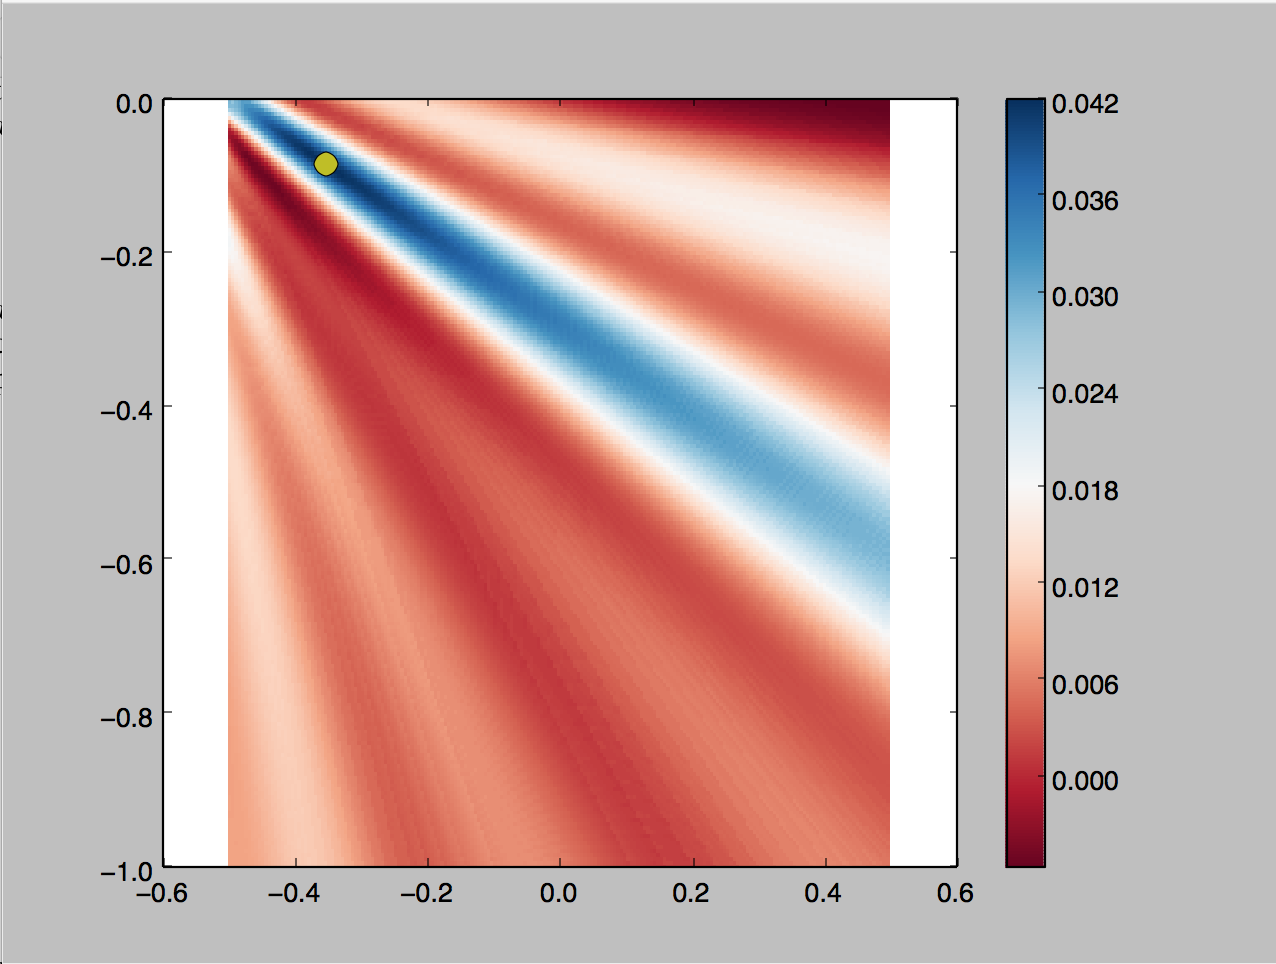
\includegraphics[width=\textwidth]{left.png}
    \caption{localization with only array 1}
    \label{fig:liklihood1}
  \end{subfigure}
  \begin{subfigure}[]{.48\textwidth}
    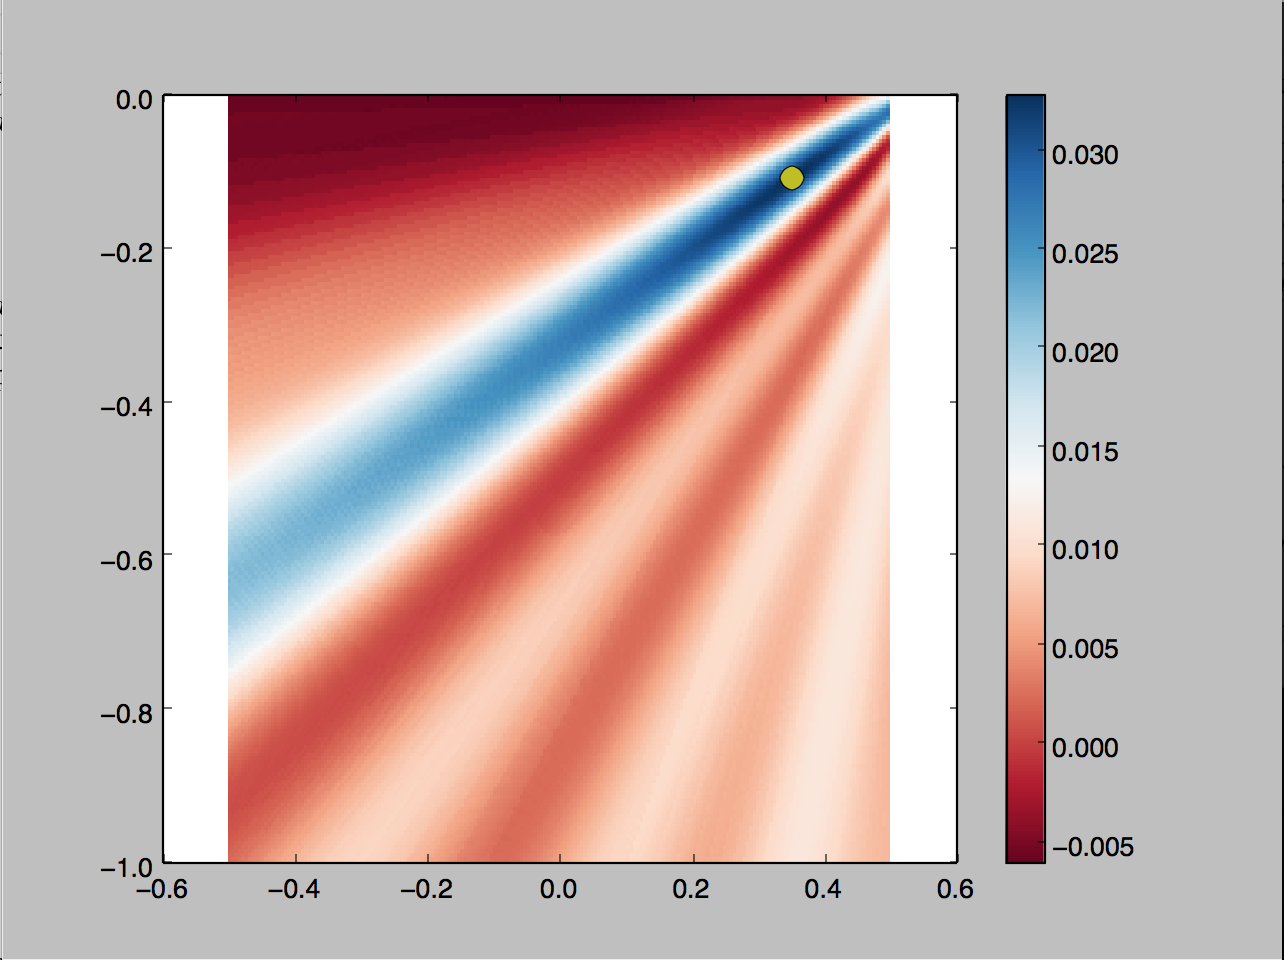
\includegraphics[width=\textwidth]{right.png}
    \caption{localization with only array 2}
    \label{fig:liklihood2}
  \end{subfigure}
  \begin{subfigure}[]{.48\textwidth}
    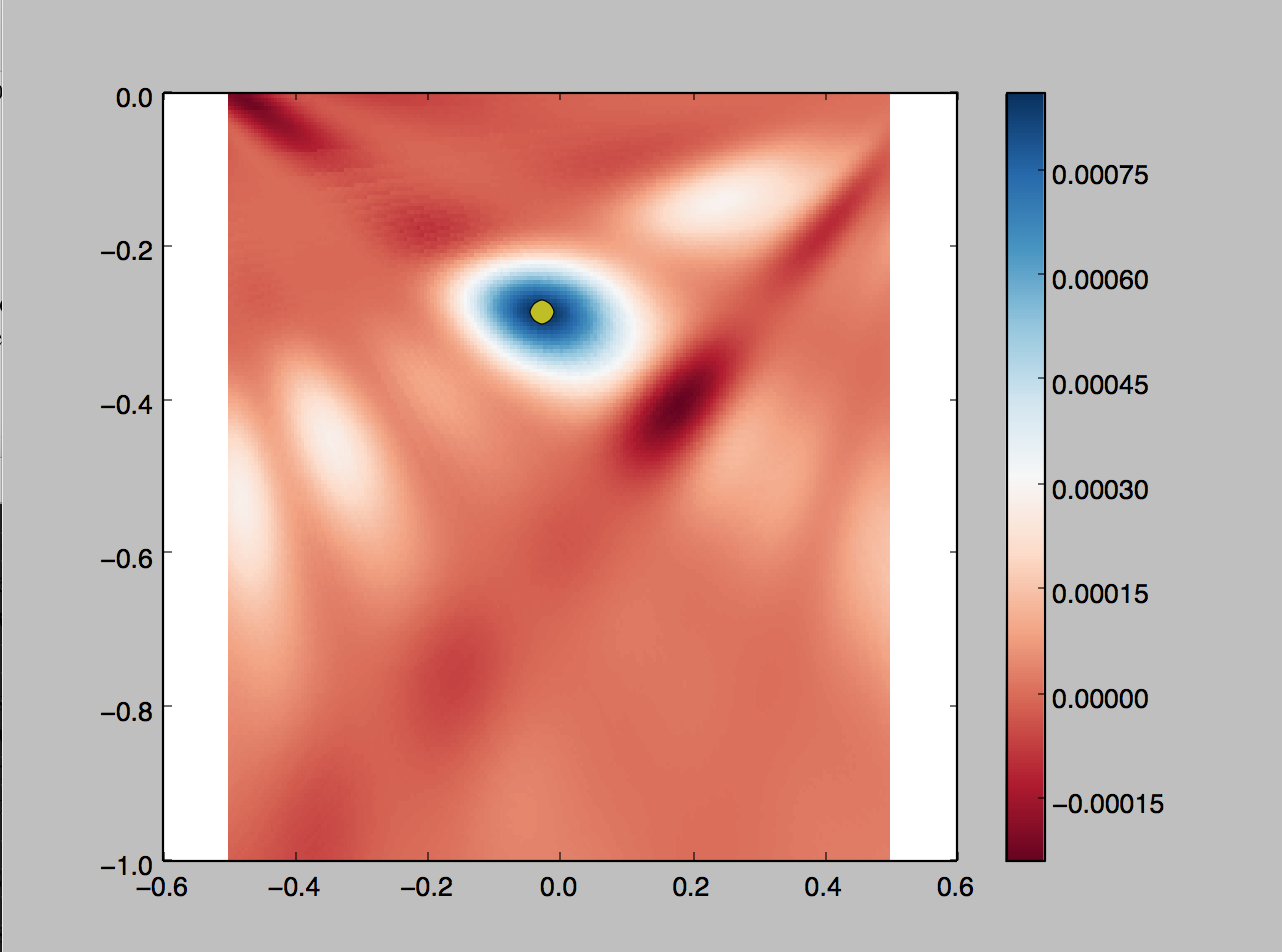
\includegraphics[width=\textwidth]{combined.png}
    \caption{localization with both arrays}
    \label{fig:liklihood3}
  \end{subfigure}
  \caption{Likelihood maps for localization. The source is placed at $(0.0,-0.3)$ m}
  \label{fig:liklihood}
\end{figure}

To see the effect of accuracy improvement using multiple arrays, fig~\ref{fig:liklihood} shows a real life localization where the source is placed at $(0$ cm$,-30$ cm$)$. The top two figures show the individual likelihood maps produced by single microphone arrays. We can see that the individual arrays can give accurate angle estimate, but have high uncertainty in distance estimate. The bottom figure shows the combined likelihood map according to equation~\ref{eq:combine_l}. The combined likelihood map demonstrated that by merging estimates from two arrays the system is able to perform more accurate localization. 


From a timing point of view, the micro-controller spends $12$ milliseconds on sampling the microphone data before sending it to a computer for processing. Sending the data through the USB port takes another $15$ milliseconds, and processing on the computer takes around $50$ milliseconds. Therefore, the total time lag between sound source and localization is around $80$ milliseconds.
